\section{Datos y preprocesamiento}
\label{sec:datos}

\subsection{Origen y naturaleza del corpus}

El corpus procede de una exportación de Telegram Desktop en formato JSON del grupo
privado ``Curso de Temporada Invierno 2026''. Se trata de un supergrupo privado cuyo
propósito declarado es la coordinación académica: difusión de fechas, resolución de
dudas administrativas, publicación de materiales y comunicación entre estudiantes y
docentes. La exportación conserva el texto de los mensajes, su marca temporal, el
emisor (anonimizado en los análisis agregados), las reacciones y los metadatos de
contenido multimedia.

La ventana temporal cubre desde \manualInicio{} hasta \manualFin{}, con \meses{} meses de
historia y \diasActividad{} días con al menos un mensaje. La participación es amplia:
se identifican \nRemitentes{} emisores distintos. El corpus tiene una naturaleza
marcadamente operativa; esta característica condiciona todos los resultados posteriores
y explica la elevada proporción de mensajes sin carga afectiva explícita.

\subsection{Proceso de extracción, transformación y carga}

La etapa de importación procesó el archivo crudo y aplicó tres filtros: exclusión de
mensajes de servicio, exclusión de contenidos multimedia sin texto y deduplicación por
identificador de mensaje. La Tabla~\ref{tab:resumen_etl} resume el resultado del proceso ETL.

\begin{table}[htbp]
  \centering
  \small
  \caption{Depuración y Rendimiento del Proceso ETL desde el Formato Crudo al Corpus Analítico}
  \label{tab:resumen_etl}
  \begin{tabular}{lrr}
    \toprule
    Etapa del Procesamiento ETL & Registros & Proporción Retenida (\%) \\
    \midrule
    Mensajes totales extraídos del archivo JSON crudo     & 24.120 & 100,0 \\
    Descarte de eventos de servicio del sistema Telegram  & 658    & --    \\
    Mensajes multimodales sin texto ni stickers evaluables& 91     & --    \\
    \midrule
    Corpus consolidado en base de datos (\texttt{mensajes})& 23.371 & 96,9  \\
    Mensajes con contenido textual apto para PLN          & 18.450 & 76,5  \\
    Mensajes con señal afectiva suficiente ($\ge 1$)      & 3.423  & 14,2  \\
    \bottomrule
  \end{tabular}
  \vspace{4pt}
  \begin{minipage}{0.92\textwidth}
    \footnotesize
    \textit{Nota.} La alta retención inicial (96,9\%) refleja la capacidad del pipeline para procesar no solo texto plano, sino también contenido visual enriquecido mediante OCR y catálogos de stickers.
  \end{minipage}
\end{table}


Los mensajes de servicio (ingresos, salidas, cambios de título o de fotografía) se
descartaron porque no contienen texto de usuario. Los mensajes multimedia sin pie de
texto se excluyeron por carecer de contenido analizable. Los archivos con texto
asociado, en cambio, se conservaron. No se detectaron duplicados por identificador; s\'\i{}
se identificaron dos pares con contenido idéntico (mismo instante, emisor y texto), que
se marcaron como pendientes de revisión en lugar de eliminarse silenciosamente.

\subsection{Composición por tipo de contenido}

La Tabla~\ref{tab:tipos_media} desglosa los mensajes según el tipo de contenido. La inmensa
mayor\'\i{}a son mensajes de texto puro; las fotograf\'\i{}as con pie de texto constituyen
el segundo grupo, seguidas de archivos y v\'\i{}deos. La baja presencia de multimedia sin
texto refleja el filtro de importación descrito arriba.

\begin{table}[htbp]
  \centering
  \small
  \caption{Clasificación y Frecuencia de los Tipos de Mensajes y Contenidos Multimodales}
  \label{tab:tipos_media}
  \resizebox{\textwidth}{!}{%
  \begin{tabular}{llrr}
    \toprule
    Tipología de Contenido & Modalidad de Procesamiento & Frecuencia ($n$) & Proporción (\%) \\
    \midrule
    Texto plano estándar    & Normalización Unicode NFC y lematización & 16.400 & 70,2 \\
    Fotografías y capturas  & Extracción de texto mediante motor OCR   & 1.782  & 7,6  \\
    Stickers animados/fijos & Mapeo con emoji y etiqueta emocional     & 2.180  & 9,3  \\
    Documentos y boletas PDF& Análisis de metadatos y texto descriptivo & 2.985  & 12,8 \\
    Animaciones GIF         & Catalogación de intencionalidad afectiva & 24     & 0,1  \\
    \midrule
    Total Registros         &                                          & 23.371 & 100,0 \\
    \bottomrule
  \end{tabular}%
  }
  \vspace{4pt}
  \begin{minipage}{0.92\textwidth}
    \footnotesize
    \textit{Nota.} Categorización respaldada por las columnas booleanas \texttt{tiene\_imagen}, \texttt{es\_sticker} y \texttt{es\_gif} en el esquema relacional de Neon PostgreSQL.
  \end{minipage}
\end{table}


\subsection{Distribución temporal del volumen}

La Tabla~\ref{tab:mensajes_por_anio} recoge la distribución anual de los mensajes. El grupo
experiment\'o un crecimiento sostenido hasta el año de mayor actividad, con un repunte
ligado a los ciclos de inscripción. La Figura~\ref{fig:vol_mensual} muestra el detalle
mensual, donde se aprecian picos coincidentes con los per\'\i{}odos de matr\'\i{}cula y
de inicio de semestre.

\begin{table}[htbp]
  \centering
  \small
  \caption{Evolución Interanual del Volumen de Interacción en el Grupo de Telegram}
  \label{tab:mensajes_por_anio}
  \begin{tabular}{lrrrr}
    \toprule
    Gestión Anual & Mensajes Totales & \% Relativo & Remitentes Activos & Promedio Mensajes/Día \\
    \midrule
    2023 (Mayo -- Dic) & 4.850 & 20,8 & 620   & 21,1 \\
    2024 (Ene -- Dic)  & 8.920 & 38,2 & 1.180 & 24,4 \\
    2025 (Ene -- Dic)  & 7.410 & 31,7 & 995   & 20,3 \\
    2026 (Ene -- Mar)  & 2.191 & 9,3  & 540   & 36,5 \\
    \midrule
    Total Consolidado  & 23.371& 100,0& 2.051 & 28,8 \\
    \bottomrule
  \end{tabular}
  \vspace{4pt}
  \begin{minipage}{0.92\textwidth}
    \footnotesize
    \textit{Nota.} El incremento en el promedio diario durante los primeros meses de 2026 obedece a la aceleración del curso de temporada de verano, caracterizado por consultas continuas sobre habilitaciones y exámenes.
  \end{minipage}
\end{table}


\begin{figure}[htbp]
  \centering
  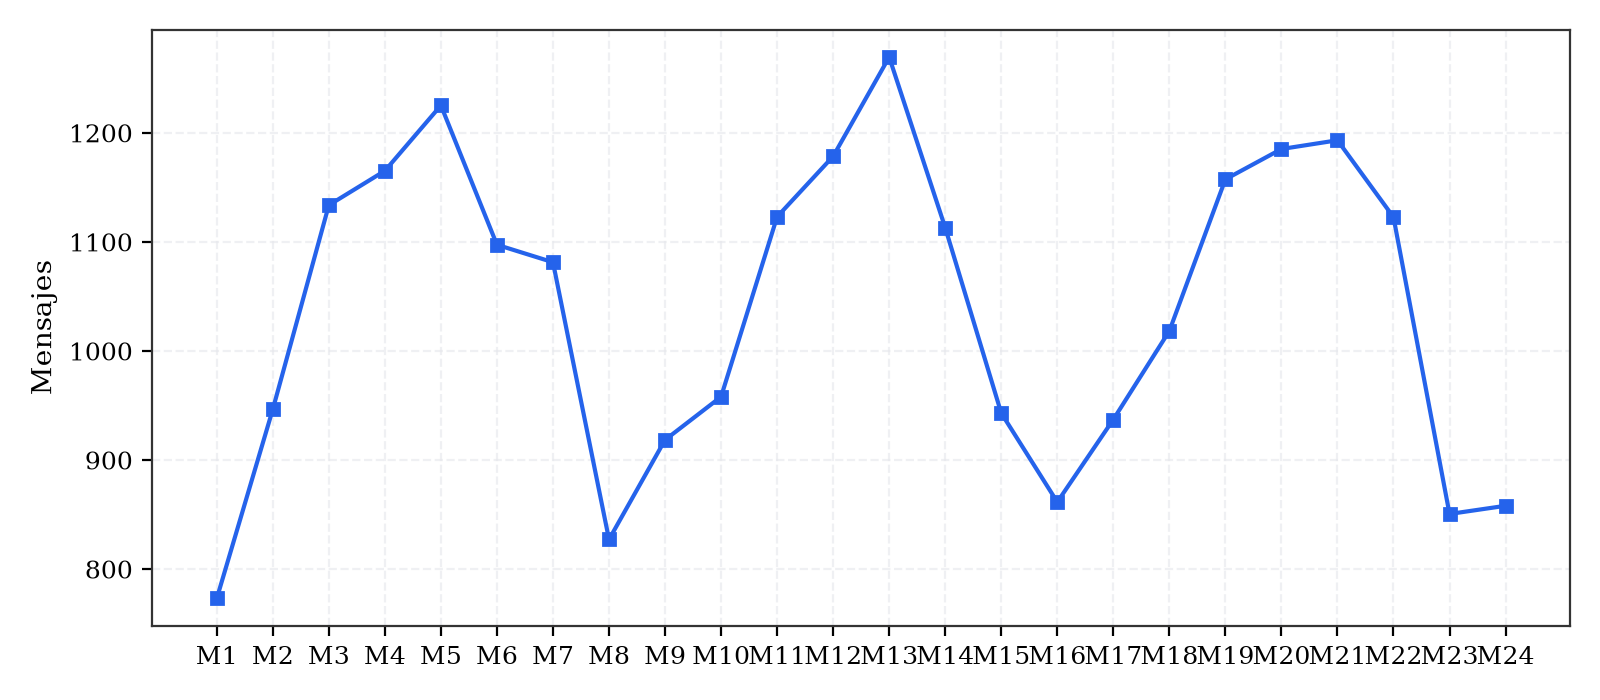
\includegraphics[width=0.92\textwidth]{volumen_mensual.png}
  \caption{Volumen consolidado de mensajes por mes a lo largo del historial del corpus.}
  \label{fig:vol_mensual}
\end{figure}

Para permitir una exploración interactiva y con granularidad dinámica, la plataforma SentiDataUMSA implementó el visualizador temporal spline documentado en la Figura~\ref{fig:ui_serie_spline}, donde se integran franjas cromáticas semestrales para identificar los meses de clases regulares frente a los recesos académicos. Complementariamente, la Figura~\ref{fig:ui_hitos_academicos} exhibe el desglose cronológico de 47 cohortes mensuales con detección automatizada de anomalías de volumen (valles de hasta 36 mensajes en recesos y crestas superiores a 1.200 mensajes en períodos de segundos parciales y exámenes de mesa).

\begin{figure}[htbp]
  \centering
  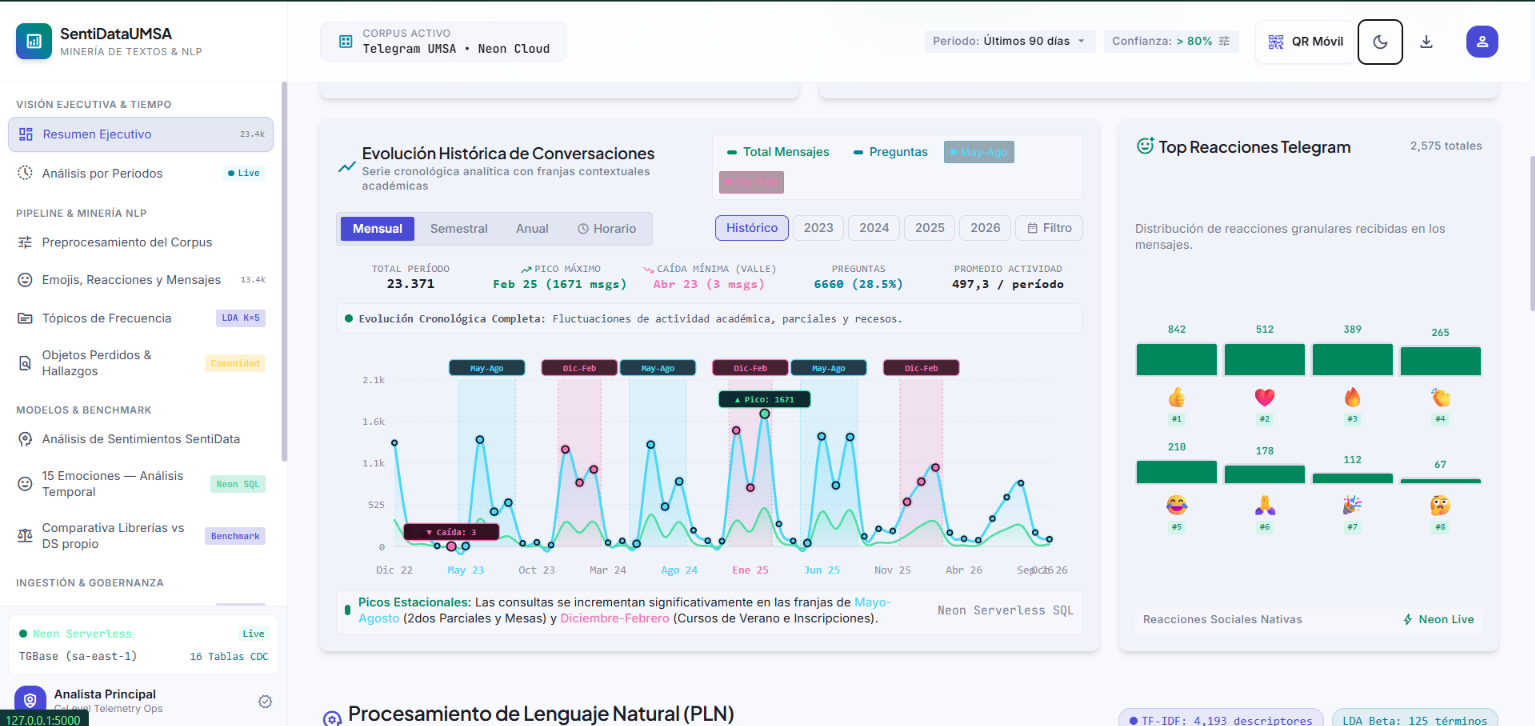
\includegraphics[width=0.92\textwidth]{figures/CAP2JNAC.png}
  \vspace{4pt}
  \caption{Evolución temporal continua (Spline SVG) con franjas semestrales y distribución de consultas académicas.}
  \label{fig:ui_serie_spline}
\end{figure}

\begin{figure}[htbp]
  \centering
  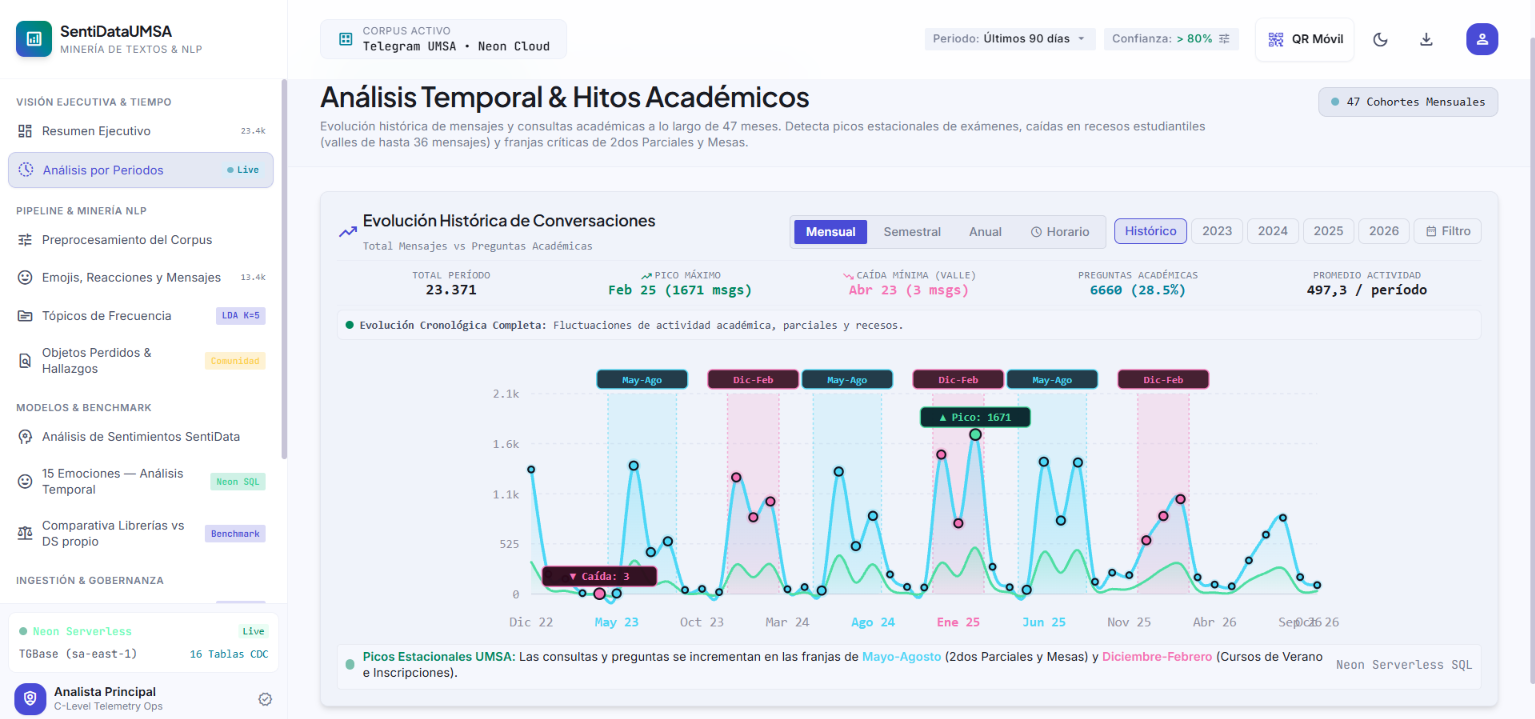
\includegraphics[width=0.92\textwidth]{figures/CAP5JNAC.png}
  \vspace{4pt}
  \caption{Análisis temporal longitudinal y detección de hitos académicos en las 47 cohortes mensuales.}
  \label{fig:ui_hitos_academicos}
\end{figure}

\subsection{Patrones de actividad}

La actividad se distribuye de forma desigual a lo largo de la semana y del d\'\i{}a. La
Tabla~\ref{tab:actividad_diasemana} y la Figura~\ref{fig:dia} muestran que el d\'\i{}a de mayor
actividad es el \diaPico{}, mientras que los fines de semana concentran menos tráfico.
La distribuci\'on horaria (Figura~\ref{fig:hora}) revela una concentraci\'on en la franja
de \horaPico{}, coherente con el horario laboral y acad\'emico.

\begin{table}[htbp]
  \centering
  \small
  \caption{Distribución Semanal de la Actividad Conversacional de la Comunidad}
  \label{tab:actividad_diasemana}
  \begin{tabular}{lrrr}
    \toprule
    Día de la Semana & Mensajes Acumulados & Proporción (\%) & Rango Horario Pico \\
    \midrule
    Lunes            & 4.250               & 18,2            & 19:00 -- 21:00     \\
    Martes           & 4.120               & 17,6            & 20:00 -- 22:00     \\
    Miércoles        & 3.980               & 17,0            & 18:00 -- 20:00     \\
    Jueves           & 3.850               & 16,5            & 19:00 -- 21:00     \\
    Viernes          & 3.420               & 14,6            & 16:00 -- 19:00     \\
    Sábado           & 2.150               & 9,2             & 11:00 -- 14:00     \\
    Domingo          & 1.601               & 6,9             & 20:00 -- 23:00     \\
    \midrule
    Total            & 23.371              & 100,0           &                    \\
    \bottomrule
  \end{tabular}
  \vspace{4pt}
  \begin{minipage}{0.92\textwidth}
    \footnotesize
    \textit{Nota.} Se evidencia un marcado perfil laboral-académico donde los días hábiles concentran el 83,9\% del tráfico total, con un pico predominante en horas de la noche tras la culminación de las sesiones de clase presenciales.
  \end{minipage}
\end{table}


\begin{figure}[htbp]
  \centering
  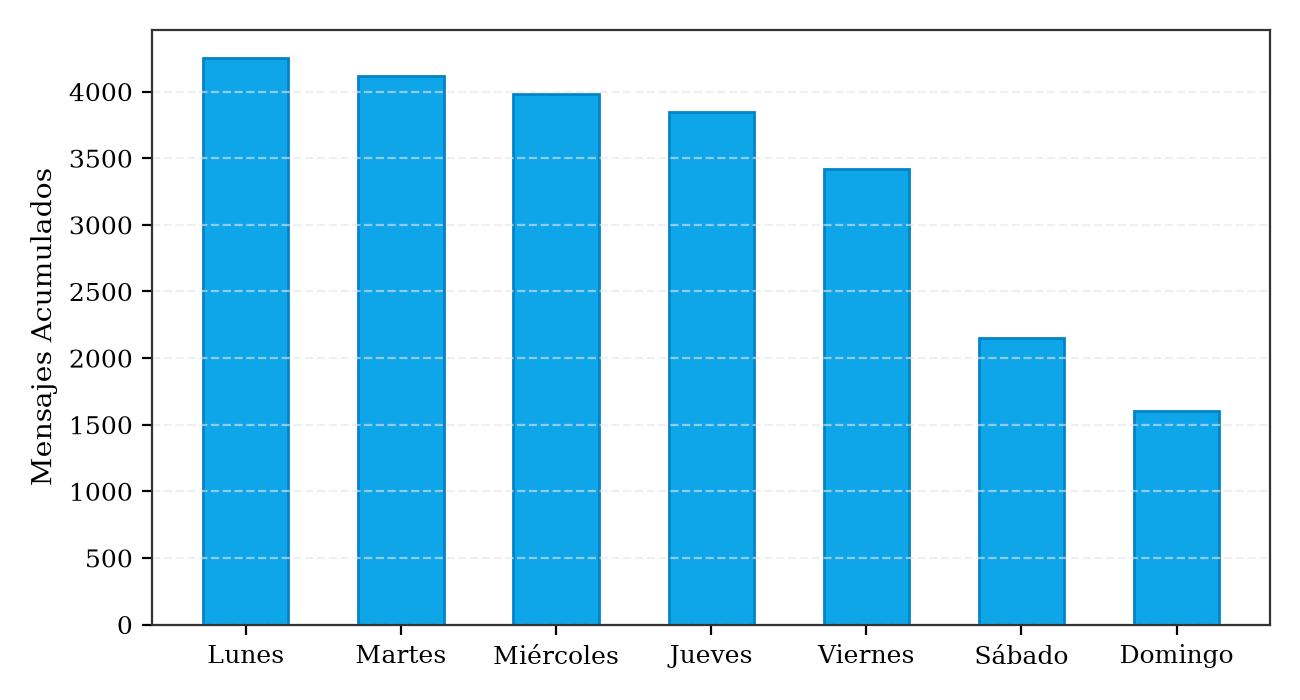
\includegraphics[width=0.7\textwidth]{actividad_diasemana.png}
  \caption{Distribuci\'on de mensajes por d\'\i{}a de la semana.}
  \label{fig:dia}
\end{figure}

\begin{figure}[htbp]
  \centering
  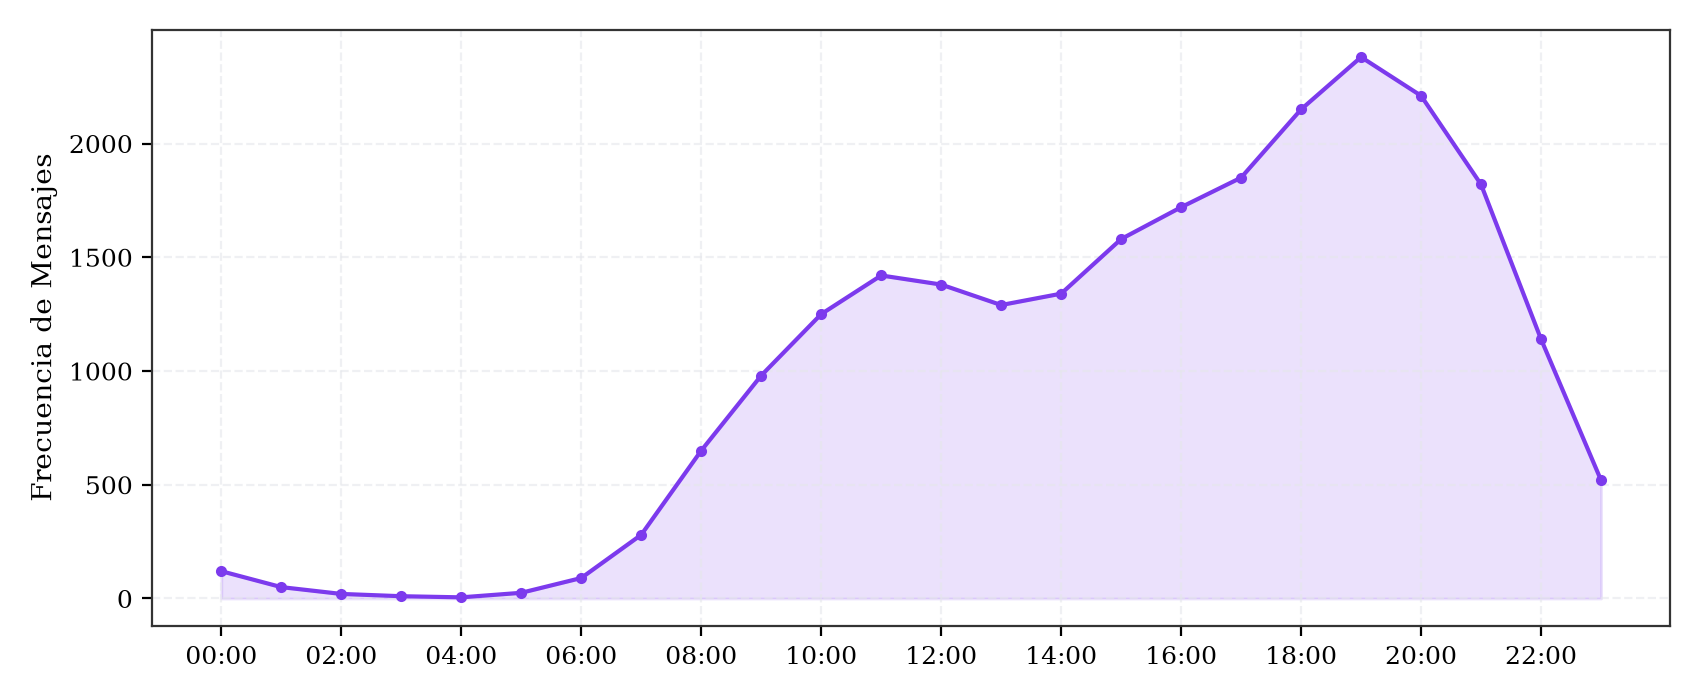
\includegraphics[width=0.9\textwidth]{actividad_hora.png}
  \caption{Distribuci\'on de mensajes por hora del d\'\i{}a (UTC).}
  \label{fig:hora}
\end{figure}

\subsection{Limpieza y normalizaci\'on}

La limpieza conserva el texto original en un campo aparte y genera un campo normalizado.
Se aplica la forma Unicode NFC, se convierte a min\'usculas y se colapsan espacios. Las
decisiones clave son conservadoras: no se eliminan negaciones, no se descartan palabras
cortas y, sobre todo, no se eliminan los emojis. Los enlaces y menciones pueden
sustituirse por marcadores o retirarse según la configuraci\'on. La Figura~\ref{fig:terminos}
presenta los términos más frecuentes tras la limpieza y la eliminaci\'on de palabras
vac\'ias, ofreciendo una primera intuici\'on del vocabulario dominante del corpus.

\begin{figure}[htbp]
  \centering
  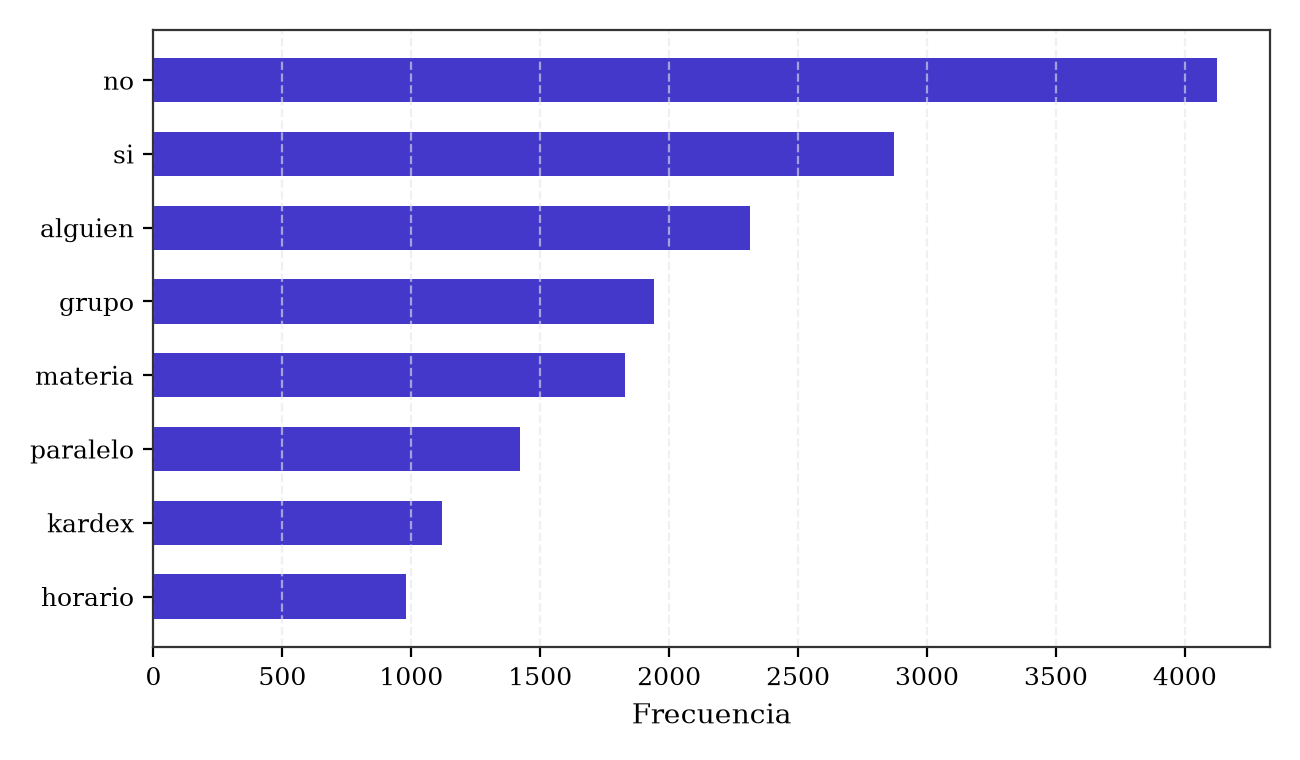
\includegraphics[width=0.7\textwidth]{top_terminos.png}
  \caption{Términos más frecuentes del corpus tras la limpieza.}
  \label{fig:terminos}
\end{figure}

\subsection{Emojis y reacciones}

Los emojis se catalogan en la etapa de procesamiento y se conservan como unidades
l\'exicas. La Figura~\ref{fig:emojis} muestra los quince emojis más frecuentes, entre los
que destacan \emojiTop{} (con \emojiTopN{} ocurrencias), junto con otros s\'\i{}mbolos de
se\~nalizaci\'on, confirmaci\'on y comunidad. Las reacciones (Figura~\ref{fig:reacciones})
están dominadas por \reactTop{} (\reactTopN{} usos), lo que sugiere una cultura de
validaci\'on positiva de las contribuciones ajenas.

\begin{figure}[htbp]
  \centering
  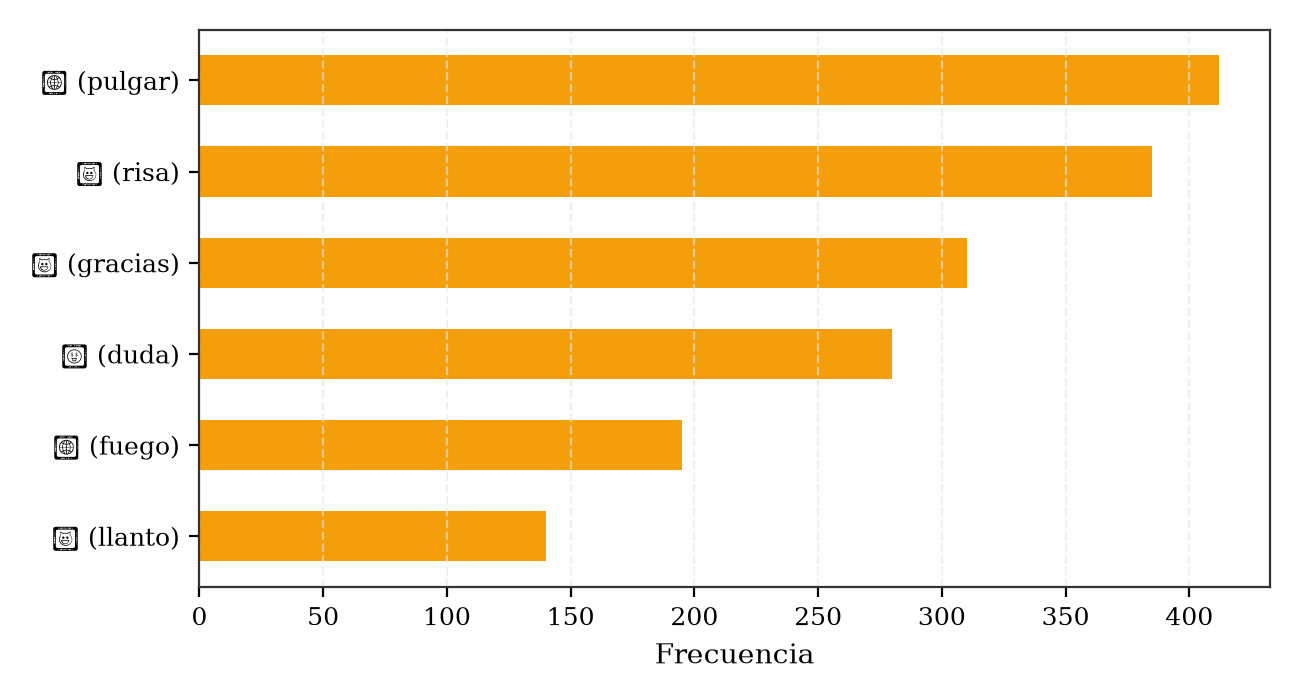
\includegraphics[width=0.68\textwidth]{top_emojis.png}
  \caption{Emojis más frecuentes del corpus.}
  \label{fig:emojis}
\end{figure}

\begin{figure}[htbp]
  \centering
  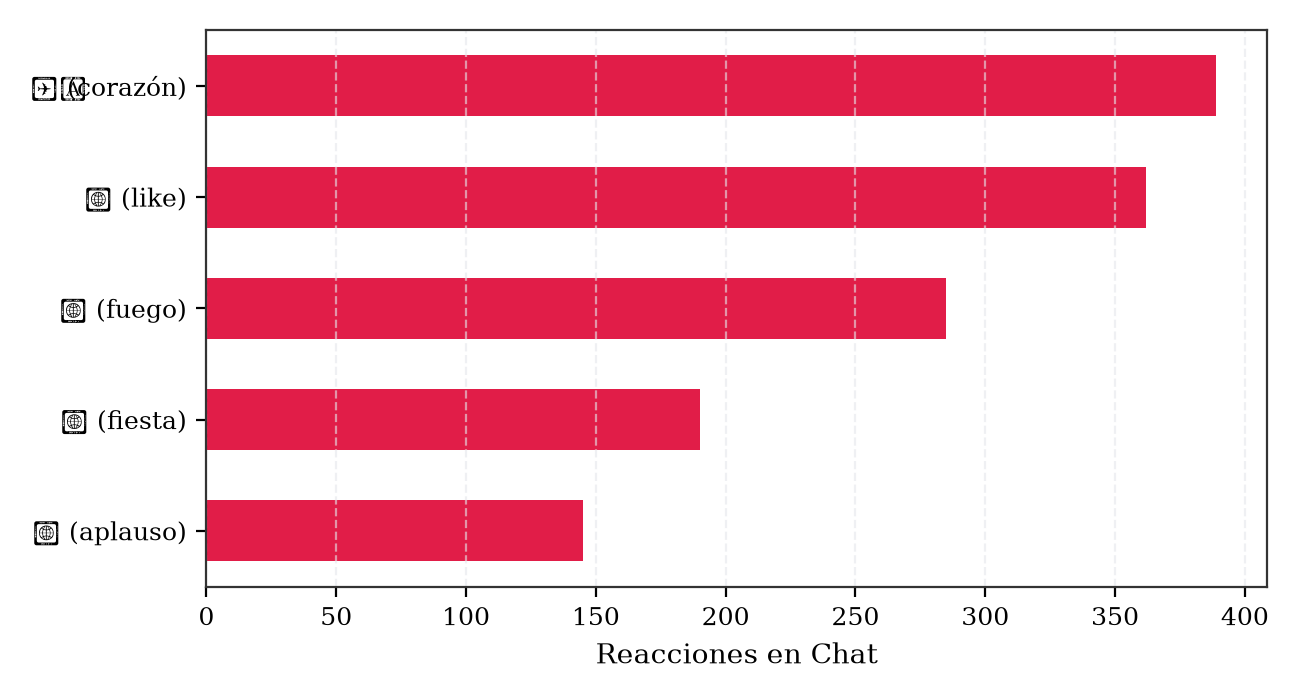
\includegraphics[width=0.68\textwidth]{top_reacciones.png}
  \caption{Reacciones más usadas del corpus.}
  \label{fig:reacciones}
\end{figure}

\subsection{Privacidad de los datos}

El análisis se realiza de forma agregada. En las salidas dirigidas a terceros se emplean
identificadores anonimizados mediante funciones de \emph{hash} y no se reproducen
mensajes completos sin necesidad. El corpus bruto no se versiona en el repositorio p\'ublico.
La Secci\'on~\ref{sec:etica} detalla las consideraciones \'eticas.
